\subsection{Bài 5: Multi}
Hàm \texttt{multi(x1n, x1origin, x2n, x2origin)} thực hiện phép nhân từng mẫu giữa hai tín hiệu:
\[
y(n) = x_1(n) \cdot x_2(n)
\]
\begin{itemize}
    \item \textbf{Đầu vào:} Hai vector tín hiệu \texttt{x1n}, \texttt{x2n} và gốc thời gian tương ứng \texttt{x1origin}, \texttt{x2origin}.
    \item \textbf{Đầu ra:} Vector kết quả \texttt{yn}, vị trí gốc thời gian mới \texttt{yorigin}.
\end{itemize}

\noindent\textbf{Thực thi:}\\
Cho hai tín hiệu:
\begin{itemize}
    \item $x_1(n) = \{1, \underset{\uparrow}{2}, 3, 4\}$, $x1origin = 2$ ($n \in [-1, 2]$)
    \item $x_2(n) = \{\underset{\uparrow}{2}, 1, -1\}$, $x2origin = 1$ ($n \in [0, 2]$)
\end{itemize}
Gọi hàm: \texttt{[yn, yorigin] = multi([1, 2, 3, 4], 2, [2, 1, -1], 1)}
\begin{itemize}
    \item Miền thời gian chung: $n \in [-1, 2]$
    \item Kết quả: \texttt{yn = [0, 4, 3, -4]}, \texttt{yorigin = 2}
    \item Giải thích: Tại $n = -1$, do $x_2(-1) = 0$ nên $y(-1) = 1 \cdot 0 = 0$. Tại các điểm giao nhau $n = 0, 1, 2$, giá trị của $y(n)$ lần lượt là $2 \cdot 2 = 4$, $3 \cdot 1 = 3$, $4 \cdot (-1) = -4$.
\end{itemize}

\begin{figure}[H]
    \centering
    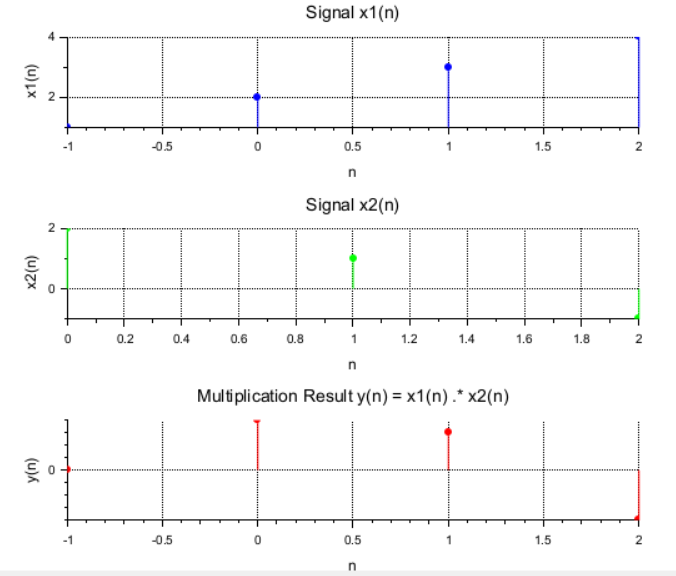
\includegraphics[width=0.65\textwidth]{img/ex5.png}
    \caption{Đồ thị tín hiệu $x_1(n)$, $x_2(n)$ và kết quả phép nhân $y(n) = x_1(n) \cdot x_2(n)$}
\end{figure}

\noindent$\rightarrow$ \textbf{Nhận xét:} Hàm tự động căn chỉnh vùng thời gian chung và thực hiện phép nhân từng cặp mẫu tương ứng một cách chính xác.
